\section{Architecture}
Before diving into the code and its structure, let's take the time to understand how the developers worked. Until \doom, everything was done on a PC. Code was written, compiler generated an executable which ran on the same machine. With the introduction of \NeXT workstations, things had to be different.\\
\par
A developer had two machines, a workstation and a PC. All work was done on the \NeXT. Code was written, compiled and ran using \fixme{Text.app} and \cw{gcc/ld}.\\
\par
Only once the developer was happy with the result, he switched to his second machine. In order to do so, he litteraly rolled his chair to the PC where the \NeXT workstation hard-drive was mounted over NFS. On this side, the PC compiled the same source code\footnote{With some platform specifics.} using \cw{WATCOM.EXE} which generated \cw{DOOM.EXE} and ran it to assess performances and playtest.\\
\par
 In this setup the PC harddrive was used to boot the machine and host the compiler. Everything else was stored on the \NeXT SCSI HDD.\\
\par
There were significant obstacle to sharing the source code. First of all, DOS program had direct access to the hardware whereas NeXT process had to use "official" APIs. Second and perhaps most importantly, the two machines had different endianess. A PC had Intel CPU which are little endian, while \NeXT was using Motorola 68040 CPU which were big endian.\\
\par
\begin{figure}[H]
\centering
\scaleddrawing{0.7}{dev_setup}{Next HDD is mounted on DOS machine on Z drive.}
\end{figure}
\par



\subsection{Endianees}
A stream of byte can be interpreted differently based on the machine internal architecture. The stream \cw{0x12}, \cw{0x34}, \cw{0x45}, \cw{0x78} can be interpreted in two ways. On a little endian machine, it will be read as \cw{0x78563412}. On a big endian machine, it will be read \cw{01234567}.\\
\par
\spngdrawing{0.5}{endianness}{}
\par
In the source code this issue could easily be solved with a simple macro.\\
\par
\ccode{big_little_endian.c}
\par
Even though \doom was written on a \NeXT the platform would always put itself at a disadvantage because players would use MS-DOS. Data was written in little endian so \cw{LONG} was a no-op on consumer hardware.\\
\par
\ccode{LongSwap.c}
\par
Accomodating the needs of running on different architecture was more challenging. The solution id programmers came up with was to have a "kernel" common to all platforms tapping into sub-systems specific to the hardware they supported.\\
\par
\begin{figure}[H]
\centering
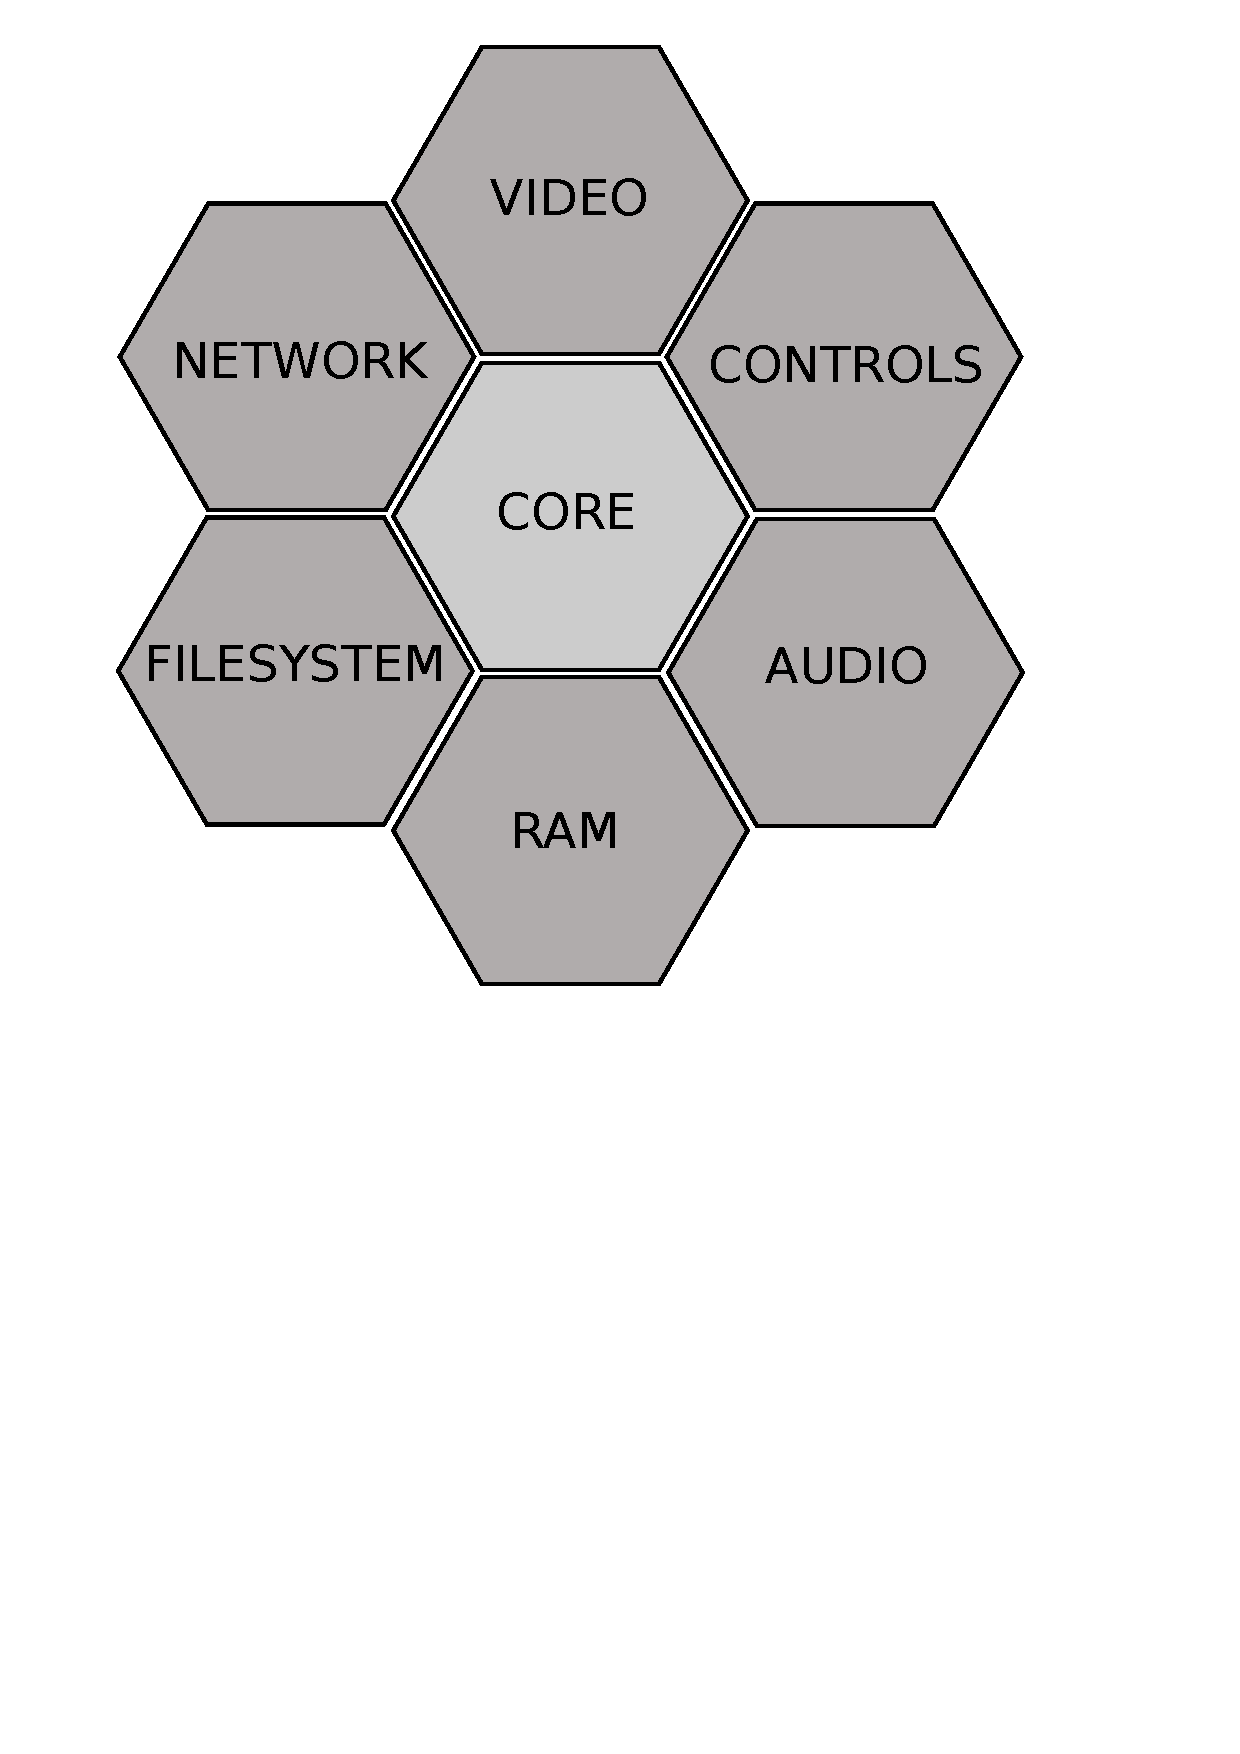
\includegraphics[width=.5\textwidth]{drawings/doom_arch.pdf}
\caption{Doom kernel and its I/O platform-dependent systems.}
\end{figure}
\par

To implement this kenel/systems architecture, they leveraged the C compiler linker. While building a C program, all compilation units (\cw{.c} files) are compiled in sequence to generate \cw{obj} files. At this stage, all symbols need not to be resolved. Taking the example of \cw{s\_sound.c}, this translation unit can use function such as \cw{I\_PlaySong} or \cw{I\_StartSound} which are defined somewhere else. \\
\par
\tcode{s_sound_linker.txt}
\par
Only when the linker runs to combine all \cw{obj} file into the final executable, all symbols have to be resolved.\\
\par
DRAWING\\
\pagebreak






\fullimage{Doom_build_NeXTStep.png}
\fakedosoutput{dos_compilation.txt}
\pagebreak


\drawing{doom_code_arch}{}
\par



In grey the I/O system which require platform specific code. On DOS six extra files are compiled and linked against the kernel: \cw{i\_main.c}, \cw{i\_ibm.c}, \cw{planar.asm}, \cw{i\_ibm\_a.asm}, \cw{i\_sound.c} and, \cw{i\_cyber.c}.\\
\par
\trivia{Notice the prefix. \cw{G\_} = blabla, \cw{I\_} is for "Implemention specific" etc...}\\

The beauty of this architecture is that once the platform specific systems are written, there is zero overheard to writing code running on multiple platform. Most of the code goes into the kernel and the platform specific code needs not to be touched anymore.
\par



\section{Structure of the code}
The volume of code is twice as much as Wolfenstein 3D.\\
\par
\tcode{cloc.txt}
\par
\trivia{The MS-DOS source code features what should have been a Doom easter egg. Files \cw{am\_oids.h} and \cw{am\_oids.c} were to allow player to play a remake of Asteroids in the automap but was left unfinished.}\\
\par
\fq{I can't recall whose idea it was, but it was probably mine.  I was taken by the vector art style of the automap, so Asteroids would have been a good fit, but Doom was behind, and the pace of development at id was incredibly fast.}{Dave Taylor}\\
\par
\pagebreak



\trivia{\NeXT platform specific were all written in Objective-C: \cw{DRCoord.m}, \cw{VGAView.m}, \cw{Doom\_main.m}, \cw{i\_next.m}, \cw{r\_debug.m},  }\\
\par
 \begin{figure}[H]
\centering  
\begin{tabularx}{\textwidth}{ L{0.22} | C{0.39} | C{0.39} }
  \toprule
  \textbf{System} & \textbf{DOS Implementation} & \textbf{NeXT Implementation}\\
  \toprule 
    Video System & VGA & \fixme{X} \\
    Audio System & DMX & Not Implemented\\
    Control System & DMPI Interrupts & \fixme{X} \\
    File  System & Direct & BigEndian converter\\
    Network System & \fixme{X} & \fixme{X} \\
   \toprule
\end{tabularx}
\caption{Platform code specific.}
\end{figure}

\par


The \cw{main} function can be found in \cw{i\_main.c} translation unit. It jumps right into \cw{D\_DoomMain} which initialize all systems in order.\\
\par
\ccode{main_loop.c}
\pagebreak

The function calls match exactly what players could see upon starting up \doom.\\
\par
\fakedosoutput{doom_dos_start.txt}
\par

\section{Fixed time steps}
Peeking inside \cw{D\_DoomLoop} reveals a pretty standard loop where the world is updated and then rendered to the audio and video output.\\
\par
\ccode{doomloop.c}
The method \cw{TryRunTics} will immediately catch the eye of an experience game developer.\\
\par
\ccode{TryRunTics.c}
\par
\doom engine is indeed using a fixed time step which runs at 35Hz. Under this architecture, the game renders as fast as possible. However before rendition occurs, it attemps to update the world in small fixed timeslice increment. In the case of \doom, a timeslice is 1/35\ts{th} of a second which is the equivalent of 28ms.\\
\par
\drawing{fixed}{}
\par
This design choice would end up being controversial. One one side it solved beautifully the issue of recording a game session and being able to playback on any machine. It also enabled network play and multiscreen play. On the other side, it meant that no matter how fast the renderer could run, the game would only update at 35Hz which would cap the next generation based on Pentium CPUs.\\
\par



\section{Game thread/Sound thread}
The second intersting thing in \cw{D\_DoomLoop} is \cw{S\_UpdateSounds} which give a clue on how sound is done. MS-DOS did not support process or thread. Yet video and audio must happen in parallel. As a result, the audio system was interrupt based. This is explained in the audio section on p\ref{dmx_section}\\
\drawing{three_systems}{}
\trivia{Notice the audio system is also in charge of generating heartbeat which \doom uses to pace itself and run at 35Hz.}







\section{Fixed arithemetic}
Before digging further inside the internals of the engine, a few words on how \doom performed mathematics. With floating points unavailable, did all its calculations using fixed point.\\
\par
\ccode{fixed_t.c}{}

\begin{figure}[H]
 \centering
  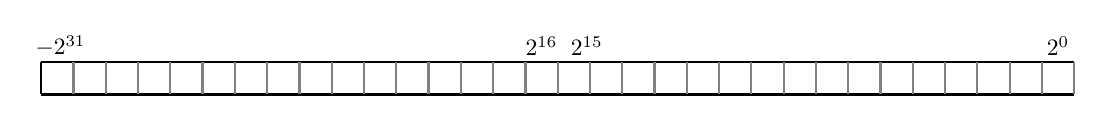
\begin{tikzpicture}[scale=0.41, every node/.style={scale=0.85}]


\colorlet{LighterMark}{black!50}

% Dark marks
\draw[thick,black] (0,0) -- (32,0);
\draw[thick,black] (0,1) -- (32,1);

\draw[thick,black] (0,1) -- (0,0);
\draw[thick,black] (32,1) -- (32,0);

% Light marks
\foreach \i in {1,...,32}
{
     \draw[thick,LighterMark] (\i,1) -- (\i,0);
}


% Labels      
\node[] at (31+0.5  ,1.5){$2^{0}$  }  ;      
\node[] at (16.5+0.4,1.5){$2^{15}$  }  ;     
\node[] at (15+0.5  ,1.5){$2^{16}$  }  ;     
\node[] at (00+0.6  ,1.5){$-2^{31}$  }  ;     


\end{tikzpicture}

 \caption{Fixed point layout 16:16 (16 bits for the integer part and 16 bits for the fractional part).} \label{fig:mips}
\end{figure}

\begin{figure}[H]
 \centering
  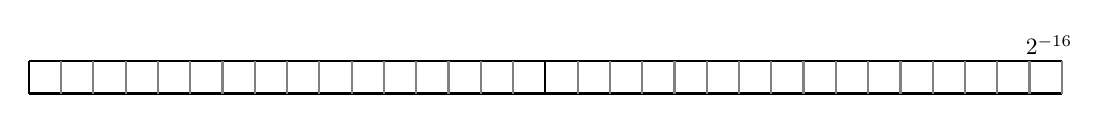
\begin{tikzpicture}[scale=0.41, every node/.style={scale=0.85}]


\colorlet{LighterMark}{black!50}

% Dark marks
\draw[thick,black] (0,0) -- (32,0);
\draw[thick,black] (0,1) -- (32,1);

\draw[thick,black] (0,1) -- (0,0);

\draw[thick,black] (32,1) -- (32,0);

% Light marks
\foreach \i in {1,...,32}
{
     \draw[thick,LighterMark] (\i,1) -- (\i,0);
}

\draw[thick,black] (16,1) -- (16,0);

% Labels      
\node[] at (31+0.6,1.5){$2^{-16}$  }  ;    
     




\end{tikzpicture}

 \caption{Fixed point layout 16:16 (16 bits for the integer part and 16 bits for the fractional part).} \label{fig:mips}
\end{figure}

\pagebreak
Bla
\pagebreak

